% Schematic representation of corona poling
% From NLO of organic molecules and polymers, Singh/Miyata.
% Author: Orlando Torres (2016)
\documentclass{standalone}

\usepackage{amsmath} % Required for \varPsi below
\usepackage{tikz,pgfplots}
\tikzset{>=latex}
\usetikzlibrary{patterns}
\begin{document}
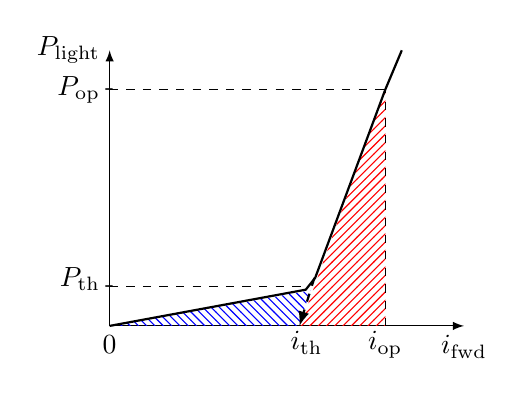
\begin{tikzpicture}

% horizontal axis
\draw[->] (0,0) -- (4.5,0) node[anchor=north] {$i_\text{fwd}$};
% labels
\draw	(0,0) node[anchor=north] {0}
		(2.5,0.05) node[anchor=north] {$i_\text{th}$}
		(3.5,0.05) node[anchor=north] {$i_\text{op}$};
% ranges
%\draw	(1,3.5) node{{\scriptsize Constant flux}}
%		(4,3.5) node{{\scriptsize Field weakening}};
\fill [draw=none, pattern=north west lines, pattern color=blue] (0,0) -- (2.40,0) -- (2.55,.45) -- cycle;
\fill [draw=none, pattern=north east lines, pattern color=red] (2.42,0) -- (3.50,0) -- (3.50,3) -- cycle;
% vertical axis
\draw[->] (0,0) -- (0,3.5) node[anchor=east] {$P_\text{light}$};
% labels
\draw	(0,0.6) node[anchor=east] {$P_\text{th}$}
		(0,0.3) node[anchor=south] {-}
		(0,3.0) node[anchor=east] {$P_\text{op}$}
		(0,2.8) node[anchor=south] {-};

		
% nominal speed
\draw[->,dashed,thick] (2.60,0.61) --(2.41,0);
\draw[dashed] (3.5,0) -- (3.5,3.0);
\draw[dashed] (0,0.5) -- (2.5,0.5);
\draw[dashed] (0,3.0) -- (3.5,3.0);
% Us
\draw[thick] (0,0) -- (2.49,0.46) -- (2.49,0.46) -- (2.61,0.61) -- (3.5,3) -- (3.71,3.5);

%\draw (1,1.5) node {$U_s$}; %label
%Y tick marks
%\foreach \x in {0,...,6}
%     		\draw (\x,1pt) -- (\x,-3pt)
%			node[anchor=north] {\x};
%    	\foreach \y in {0,...,4}
%     		\draw (1pt,\y) -- (-3pt,\y) 
%     			node[anchor=east] {\y}; 
% Psis
%\draw[thick,dashed] (0,3) -- (2,3) parabola[bend at end] (6,1);
%\draw (2.5,3) node {$\varPsi_s$}; %label

\end{tikzpicture}

\end{document}